\section{R1: Accuracy}
\label{sec:eval-r1}

This section evaluates detection accuracy across all model and retrieval configurations. The metrics are precision, recall, F1, and secure-sample false-positive rate (FPR), as defined in Section~\ref{sec:r1-accuracy}.

\subsection{Detection Quality Across Configurations}

Table~\ref{tab:eval-r1-all} shows detection metrics for all evaluated configurations. Results are pooled over 213 vulnerable-sample evaluations (71 samples $\times$ 3 runs) and 30 secure-sample evaluations.

\begin{table}[H]
\centering
\caption{Detection accuracy across all configurations.}
\label{tab:eval-r1-all}
\footnotesize
\begin{tabular}{@{}llrrrr@{}}
\toprule
\textbf{Model} & \textbf{Mode} & \textbf{Precision} & \textbf{Recall} & \textbf{F1} & \textbf{FPR} \\
\midrule
\texttt{qwen3:8b} & LLM+RAG & 63.16 & 67.61 & 65.31 & 20.00 \\
\texttt{qwen3:8b} & LLM-only & 54.65 & 66.20 & 59.87 & 40.00 \\
\texttt{qwen3:4b} & LLM+RAG & 53.53 & 64.90 & 58.67 & 100.00 \\
\texttt{qwen3:4b} & LLM-only & 51.85 & 59.29 & 54.90 & 100.00 \\
\texttt{gemma3:4b} & LLM+RAG & 47.62 & 44.25 & 45.88 & 100.00 \\
\texttt{gemma3:4b} & LLM-only & 50.00 & 47.79 & 48.87 & 100.00 \\
\texttt{gemma3:1b} & LLM+RAG & 43.75 & 24.78 & 31.65 & 100.00 \\
\texttt{gemma3:1b} & LLM-only & 45.31 & 25.66 & 32.77 & 100.00 \\
\texttt{codellama} & LLM+RAG & 46.15 & 47.79 & 46.96 & 100.00 \\
\texttt{codellama} & LLM-only & 50.91 & 49.56 & 50.22 & 100.00 \\
\midrule
\texttt{semgrep} & baseline & 57.89 & 9.73 & 16.67 & 6.67 \\
\texttt{codeql} & baseline & 15.71 & 9.73 & 12.02 & 53.33 \\
\texttt{eslint} & baseline & --- & 0.00 & 0.00 & 0.00 \\
\bottomrule
\end{tabular}
\end{table}

Figure~\ref{fig:r1-f1-comparison} visualizes the F1 scores across configurations.

\begin{figure}[H]
\centering
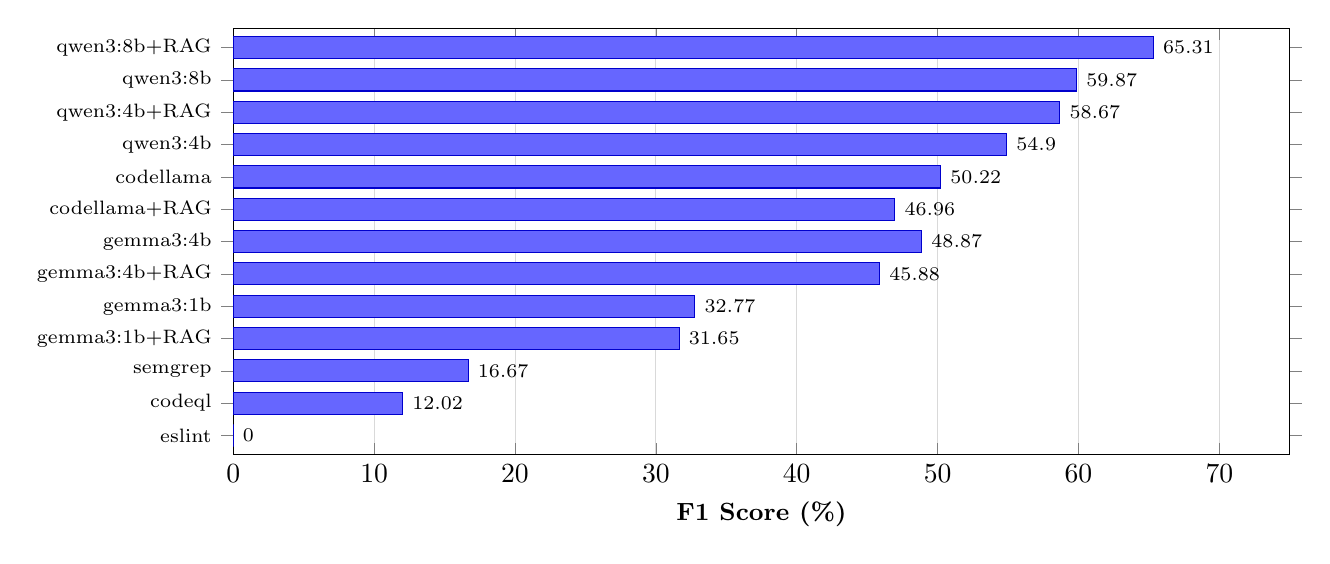
\begin{tikzpicture}
  \begin{axis}[
    width=15cm,
    height=7cm,
    xbar,
    bar width=8pt,
    xlabel={F1 Score (\%)},
    xlabel style={font=\small\bfseries},
    ylabel style={font=\small\bfseries},
    symbolic y coords={
      {eslint},
      {codeql},
      {semgrep},
      {gemma3:1b+RAG},
      {gemma3:1b},
      {gemma3:4b+RAG},
      {gemma3:4b},
      {codellama+RAG},
      {codellama},
      {qwen3:4b},
      {qwen3:4b+RAG},
      {qwen3:8b},
      {qwen3:8b+RAG}
    },
    ytick=data,
    yticklabel style={font=\scriptsize},
    xmin=0, xmax=75,
    xtick={0,10,20,30,40,50,60,70},
    xmajorgrids=true,
    grid style={line width=0.3pt, draw=gray!30},
    enlarge y limits=0.05,
    nodes near coords,
    nodes near coords style={font=\scriptsize, anchor=west},
  ]

  \addplot[fill=blue!60, draw=blue!80!black] coordinates {
    (0.00,{eslint})
    (12.02,{codeql})
    (16.67,{semgrep})
    (31.65,{gemma3:1b+RAG})
    (32.77,{gemma3:1b})
    (45.88,{gemma3:4b+RAG})
    (48.87,{gemma3:4b})
    (46.96,{codellama+RAG})
    (50.22,{codellama})
    (54.90,{qwen3:4b})
    (58.67,{qwen3:4b+RAG})
    (59.87,{qwen3:8b})
    (65.31,{qwen3:8b+RAG})
  };

  \end{axis}
\end{tikzpicture}
\caption{F1 scores across all configurations. LLM-based approaches outperform SAST baselines on recall-driven F1, with \texttt{qwen3:8b+RAG} achieving the highest score.}
\label{fig:r1-f1-comparison}
\end{figure}

\subsection{RAG Ablation Impact on Accuracy}

RAG effects are model-dependent. Figure~\ref{fig:r1-rag-ablation} compares LLM-only and LLM+RAG F1 for each model.

\begin{figure}[H]
\centering
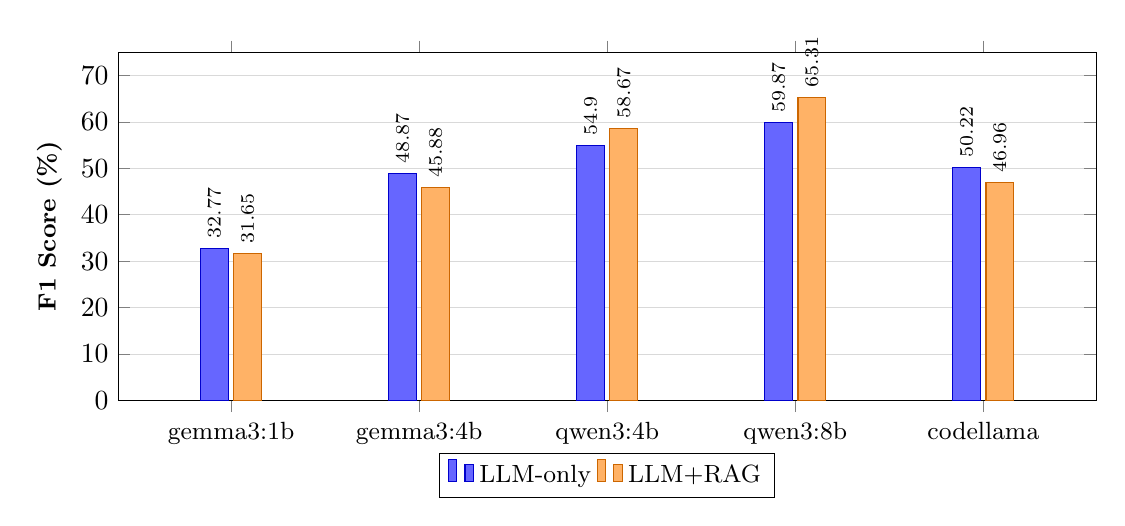
\begin{tikzpicture}
  \begin{axis}[
    width=14cm,
    height=6cm,
    ybar,
    bar width=10pt,
    ylabel={F1 Score (\%)},
    ylabel style={font=\small\bfseries},
    xlabel={Model},
    xlabel style={font=\small\bfseries},
    symbolic x coords={gemma3:1b, gemma3:4b, qwen3:4b, qwen3:8b, codellama},
    xtick=data,
    xticklabel style={font=\small},
    ymin=0, ymax=75,
    ytick={0,10,20,30,40,50,60,70},
    ymajorgrids=true,
    grid style={line width=0.3pt, draw=gray!30},
    legend style={
      at={(0.5,-0.15)},
      anchor=north,
      legend columns=2,
      font=\small,
    },
    enlarge x limits=0.15,
    nodes near coords,
    nodes near coords style={font=\scriptsize, rotate=90, anchor=west},
  ]

  \addplot[fill=blue!60, draw=blue!80!black] coordinates {
    (gemma3:1b, 32.77)
    (gemma3:4b, 48.87)
    (qwen3:4b, 54.90)
    (qwen3:8b, 59.87)
    (codellama, 50.22)
  };
  \addlegendentry{LLM-only}

  \addplot[fill=orange!60, draw=orange!80!black] coordinates {
    (gemma3:1b, 31.65)
    (gemma3:4b, 45.88)
    (qwen3:4b, 58.67)
    (qwen3:8b, 65.31)
    (codellama, 46.96)
  };
  \addlegendentry{LLM+RAG}

  \end{axis}
\end{tikzpicture}
\caption{RAG ablation: F1 comparison by model. RAG improves \texttt{qwen3} models but degrades \texttt{gemma3} and \texttt{codellama}.}
\label{fig:r1-rag-ablation}
\end{figure}

RAG improves \texttt{qwen3:8b} by +5.44 F1 points and \texttt{qwen3:4b} by +3.77 points. However, \texttt{gemma3:4b} drops by $-2.99$ points and \texttt{codellama} by $-3.26$ points with RAG enabled. This confirms that retrieval augmentation is not universally beneficial and should be treated as a model-specific configuration.

\paragraph{Statistical power.} The observed F1 differences are descriptive measurements from a single evaluation run. Exploratory exact McNemar tests on matched sample-level detection outcomes (LLM-only vs.\ LLM+RAG for each model) did not reach statistical significance for the \texttt{qwen3} improvements in this dataset ($n = 71$ vulnerable samples). This is consistent with the modest sample size: a 5-point F1 difference requires a substantially larger evaluation set to detect reliably. The RAG effect should therefore be interpreted as an indicative trend rather than a confirmed improvement, and the direction of the effect (positive for \texttt{qwen3}, negative for \texttt{gemma3} and \texttt{codellama}) is more robust than the precise magnitude.

\subsection{Per-Category Detection Breakdown}

Figure~\ref{fig:r1-category} shows recall by vulnerability category for the best configuration (\texttt{qwen3:8b+RAG}), restricted to categories with at least 3 test cases. The $n$ value indicates the number of vulnerable samples per category.

\begin{figure}[H]
\centering
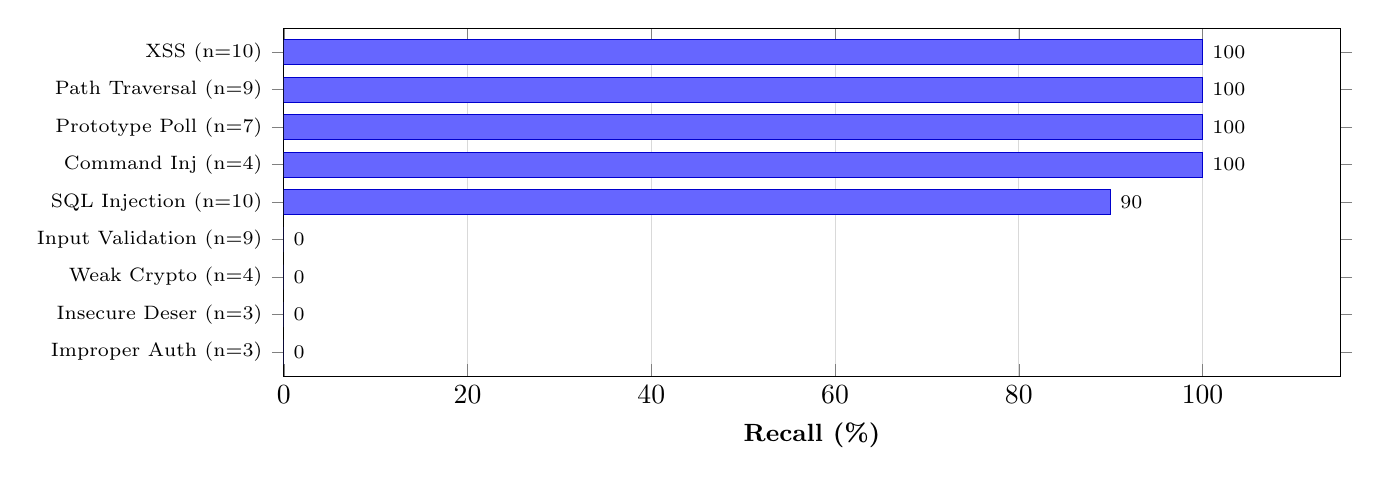
\begin{tikzpicture}
  \begin{axis}[
    width=15cm,
    height=6cm,
    xbar,
    bar width=9pt,
    xlabel={Recall (\%)},
    xlabel style={font=\small\bfseries},
    symbolic y coords={
      {Improper Auth (n=3)},
      {Insecure Deser (n=3)},
      {Weak Crypto (n=4)},
      {Input Validation (n=9)},
      {SQL Injection (n=10)},
      {Command Inj (n=4)},
      {Prototype Poll (n=7)},
      {Path Traversal (n=9)},
      {XSS (n=10)}
    },
    ytick=data,
    yticklabel style={font=\scriptsize},
    xmin=0, xmax=115,
    xtick={0,20,40,60,80,100},
    xmajorgrids=true,
    grid style={line width=0.3pt, draw=gray!30},
    enlarge y limits=0.08,
    nodes near coords,
    nodes near coords style={font=\scriptsize, anchor=west},
  ]

  \addplot[fill=blue!60, draw=blue!80!black] coordinates {
    (0,{Improper Auth (n=3)})
    (0,{Insecure Deser (n=3)})
    (0,{Weak Crypto (n=4)})
    (0,{Input Validation (n=9)})
    (90,{SQL Injection (n=10)})
    (100,{Command Inj (n=4)})
    (100,{Prototype Poll (n=7)})
    (100,{Path Traversal (n=9)})
    (100,{XSS (n=10)})
  };

  \end{axis}
\end{tikzpicture}
\caption{Per-category recall for \texttt{qwen3:8b+RAG}, showing categories with $n \geq 3$ test cases. The results reveal a bimodal pattern: injection-style categories achieve 90--100\% recall, while categories requiring semantic reasoning (validation, authentication, cryptography) achieve 0\%.}
\label{fig:r1-category}
\end{figure}

The per-category breakdown reveals a sharp split rather than a smooth gradient. Categories with well-known syntactic signatures --- injection sinks (SQL, XSS, command injection), path traversal, and prototype pollution --- are detected at 90--100\% recall. In contrast, categories where the vulnerability is the \emph{absence} of a required check rather than the presence of a dangerous pattern --- input validation, authentication, cryptographic misuse, and deserialization --- achieve 0\% recall in this dataset. This suggests that the model reliably recognizes taint-to-sink patterns but struggles when detection requires reasoning about missing logic. Per-category sample sizes range from 3 to 10, so individual percentages should be interpreted cautiously; categories with fewer than 3 samples are excluded from this figure.

\subsection{SAST Baseline Comparison}

SAST tools show a different trade-off profile. Semgrep achieves low FPR (6.67\%) but very low recall (9.73\%). CodeQL has higher FPR (53.33\%) with similarly low recall. ESLint security plugins detect none of the test cases. The LLM-based approach trades higher FPR for substantially better recall, making it more suitable for comprehensive security audits while SAST remains useful as a low-noise complement.

\subsection{Level Mapping}

Based on the R1 evaluation scale (Table~\ref{tab:r1-accuracy-thresholds}), the best configuration (\texttt{qwen3:8b+RAG}) maps as follows:

\begin{itemize}
  \item F1 = 65.31\% $\rightarrow$ falls in $[0.60, 0.75)$
  \item Precision = 63.16\% $\rightarrow$ above 0.55
  \item Recall = 67.61\% $\rightarrow$ above 0.55
  \item FPR = 20.00\% $\rightarrow$ at the $\leq 0.20$ boundary
\end{itemize}

\begin{center}
\begin{tabular}{cc}
\raisebox{-0.3cm}{\tikz{\filldraw[fill=black] (0,0) -- (90:0.35cm) arc (90:-150:0.35cm) -- cycle; \draw (0,0) circle (0.35cm);}} &
\textbf{R1 Level: Medium accuracy.} \\
\end{tabular}
\end{center}

Results are worth reviewing with some manual checking needed. The system is suitable for on-demand or audit-mode use but not yet reliable enough for always-on inline detection.
